%% Computer Physics Communications -- Computer Programs in Physics (CPiP)
%% Template: cpc-cpip-template.tex (Elsevier), elsarticle class.
%% Compile: pdflatex -> bibtex -> pdflatex -> pdflatex
\documentclass[preprint,12pt]{elsarticle}

\usepackage{amsmath}
\usepackage{amssymb}
\usepackage{booktabs}
\usepackage{siunitx}
\usepackage{graphicx}
\usepackage{url}
\usepackage[colorlinks=true,linkcolor=blue,citecolor=blue]{hyperref}

\sisetup{detect-all=true}

%% Reference list used inside the Program Summary (from the CPC template).
\newcounter{bla}
\newenvironment{refnummer}{%
\list{[\arabic{bla}]}%
{\usecounter{bla}%
 \setlength{\itemindent}{0pt}%
 \setlength{\topsep}{0pt}%
 \setlength{\itemsep}{0pt}%
 \setlength{\labelsep}{2pt}%
 \setlength{\listparindent}{0pt}%
 \settowidth{\labelwidth}{[9]}%
 \setlength{\leftmargin}{\labelwidth}%
 \addtolength{\leftmargin}{\labelsep}%
 \setlength{\rightmargin}{0pt}}}
 {\endlist}

\journal{Computer Physics Communications}

\begin{document}

\setlength{\emergencystretch}{2em}

\begin{frontmatter}

\title{OBPDS 2.0: a verified one-dimensional Schr\"odinger--Poisson and
drift--diffusion solver for III--V heterostructures}

\author[a]{First Author\corref{cor}}
\author[a]{Second Author}
\cortext[cor]{Corresponding author.\\\textit{E-mail address:} author@example.edu}
\address[a]{Affiliation, City, Country}

\begin{abstract}
% ---------------------------------------------------------------------------
%  Abstract: <= 250 words, no references, no non-standard abbreviations.
% ---------------------------------------------------------------------------
We describe OBPDS 2.0, an open-source program that solves the one-dimensional
electrostatic, transport and envelope-Schr\"odinger problems of III--V
heterostructures on a single grid. It computes self-consistent band diagrams,
terminal currents, capacitances and quantised subband structure for layer
stacks that may be pseudomorphically strained. It is a modern rewrite of the
Open Band Parameters Device Simulator, which stopped at the zero-current
approximation and produced no current; the rewrite adds
drift--diffusion transport, self-consistent quantisation and strain, and keeps
the non-parabolic multi-valley statistics of the original.

The numerical content is what we report. Scharfetter--Gummel
fluxes are written in a generalised-potential form that is an identity for
arbitrary statistics; after a cancellation-free rearrangement the
equilibrium current vanishes by construction (the vanishing factor is
computed from the quasi-Fermi level itself), instead of emerging as a
difference of large numbers. The rearrangement is an algebraic identity, not
a new discretisation, and we state that distinction explicitly in
Section~\ref{sec:sg}.
In III--V materials the carrier densities inside one device span more than
twenty decades, so the discrete current in a quasi-neutral region is below the
round-off of the stored quasi-Fermi levels; the program therefore reads the
terminal current from the depletion region and reports the relative deviation
of the worst link, which tells the user when the value is arithmetic noise.
Quantisation uses the BenDaniel--Duke operator on the same grid, and strain a
closed-form Bir--Pikus Hamiltonian with spin--orbit coupling.

Every model is held to closed-form results by a test suite whose checks are
reported by kind---analytic and asymptotic limits, discrete-operator
properties, and physical-scale regression---rather than as a single
undifferentiated count, with a separate end-to-end test for the web API
contract (Section~\ref{sec:verification}). A representative bias point
converges in two Gummel sweeps and about \SI{1.5}{s}.

% ---------------------------------------------------------------------------
%  PROGRAM SUMMARY -- mandatory for CPiP articles.
% ---------------------------------------------------------------------------
\vspace{1.2em}
\noindent \textbf{PROGRAM SUMMARY}

\begin{small}
\noindent
{\em Program Title:} OBPDS 2.0 --- Open Band Parameters Device Simulator \\
{\em CPC Library link to program files:} (to be added by Technical Editor) \\
{\em Developer's repository link:} \url{https://github.com/<owner>/obpds} \\
{\em Licensing provisions:} AGPL-3.0-or-later. This program is a derivative
of OBPDS, which is distributed under the GNU Affero General Public License
v3.0; the licence is therefore retained and cannot be replaced by one of the
licences on the standard list. \\
{\em Programming language:} Python 3 (>= 3.10); JavaScript/HTML for the
browser front end \\
{\em Supplementary material:} A verification suite whose checks are
classified by kind (analytic/asymptotic, discrete-operator, and
physical-scale regression) together with a separate web-API contract test,
a comprehensive example run with its expected output, the scripts that
regenerate every figure and table of this paper (including the current
conservation, mesh-convergence and strain-sensitivity audits), and the web
front end. \\
{\em Nature of problem (approx.\ 50--250 words):}
One-dimensional band-diagram and terminal-current calculations for III--V
heterostructures couple a strongly nonlinear Poisson equation to degenerate,
non-parabolic carrier statistics and to confinement in wells a few nanometres
wide. The dynamic range is extreme: in GaAs at room temperature the intrinsic
density is $1.7\times10^{6}$~cm$^{-3}$ against a doping of
$10^{17}$--$10^{18}$~cm$^{-3}$, so electron and hole densities differ by more
than twenty decades inside one device. A solver must stay accurate where the
current carried by a quasi-neutral region corresponds to a quasi-Fermi
gradient five orders of magnitude below the round-off of the stored levels,
and must distinguish genuine confinement from a discretisation artefact. Open
implementations either stop at the zero-current approximation, in which the
quasi-Fermi levels are prescribed and no current can be computed, or cannot be
inspected and modified. \\
{\em Solution method (approx.\ 50--250 words):}
Finite-volume discretisation of $\nabla\!\cdot(\varepsilon\nabla\psi)$ on a
uniform grid with the face permittivity taken as the harmonic mean of adjacent
nodes, so that the $\varepsilon'\psi'$ term is retained at heterointerfaces.
The Poisson system is solved by Newton's method, damped along Bank--Rose
lines [3], with every row equilibrated before the solve. Drift--diffusion uses Scharfetter--Gummel fluxes [1] in a
generalised-potential form that reduces to the standard discretisation under
Boltzmann statistics and, rearranged to be cancellation-free, gives a
zero equilibrium current without subtracting nearly equal terms.
Continuity is solved by Newton with the same damping and coupled to Poisson by
Gummel iteration [2] from an analytic minority-carrier profile, so that a bias
point converges in two or three sweeps from a cold start. Confinement uses a
BenDaniel--Duke tridiagonal eigenproblem [6] with harmonic averaging of $1/m^{*}$,
populated as two-dimensional subbands plus a continuum remainder. Pseudomorphic
strain enters through a closed-form Bir--Pikus Hamiltonian [5] with spin--orbit
coupling; band parameters follow [4]. \\
{\em Additional comments including restrictions and unusual features
(approx.\ 50--250 words):}
Restrictions: one-dimensional, single temperature, drift--diffusion with
constant low-field mobilities, no hole quantisation, no exchange--correlation,
no Auger recombination, and no strain relaxation (the Matthews--Blakeslee
thickness is reported, not applied). Quantisation is applied at equilibrium
only: there is no quantum-corrected transport, so every current and
capacitance is classical. Unusual features: (i) the terminal
current is read from the depletion region and reported together with
\texttt{J\_spread}, the relative deviation of the worst discrete link, so that
a user can see when the reported value is noise;
(ii) the equilibrium current is zero by construction of the
cancellation-free flux rather than a residual of a subtraction;
(iii) every physical model is exercised against closed-form results, including
negative controls; (iv) a browser front end serves the same solver, so no
installation is needed for classroom use; (v) the program flags the cases in which its own model is invalid, for example a
layer thicker than its critical thickness; (vi) band parameters can be
calibrated per layer, which lets a reader test what a different valence-band
offset would do without editing the parameter tables.

\begin{refnummer}
\item D.~L. Scharfetter, H.~K. Gummel, IEEE Trans.\ Electron Devices 16 (1969)
      64--77.
\item H.~K. Gummel, IEEE Trans.\ Electron Devices 11 (1964) 455--465.
\item R.~E. Bank, D.~J. Rose, Numer.\ Math.\ 37 (1981) 279--295.
\item I.~Vurgaftman, J.~R. Meyer, L.~R. Ram-Mohan, J.\ Appl.\ Phys.\ 89 (2001)
      5815--5875.
\item S.~L. Chuang, Phys.\ Rev.\ B 43 (1991) 9649--9661.
\item D.~J. BenDaniel, C.~B. Duke, Phys.\ Rev.\ 152 (1966) 683--692.
\end{refnummer}
\end{small}
\end{abstract}

\begin{keyword}
Semiconductor device simulation \sep Drift--diffusion \sep
Schr\"odinger--Poisson \sep Scharfetter--Gummel discretisation \sep
Fermi--Dirac statistics \sep Pseudomorphic strain \sep Python
\end{keyword}

\end{frontmatter}

% =========================================================== 1 Introduction
\section{Introduction}
\label{sec:intro}

One-dimensional band diagrams are the working language of III--V device
design. A layer stack, a doping profile and a substrate are enough to answer
the questions that come up first: where the electrons sit, how the bands line
up, how much of the gap is taken by the conduction-band offset, how a quantum
well shifts when it is strained. Tools of this kind have existed for decades.
Bandprof~\cite{Frensley} and its descendants, including the Open Band
Parameters Device Simulator (OBPDS)~\cite{Maddox2015} that this paper starts
from, solve the nonlinear Poisson equation for a prescribed pair of
quasi-Fermi levels---the \emph{zero-current approximation}---and draw the
result~\cite{Frensley1988}. That approximation is legitimate for a band diagram and of no use for a
current--voltage curve: with the quasi-Fermi levels fixed there is no equation
from which a current could be obtained.

The gap matters because the interesting III--V structures are exactly the ones
in which the two effects the zero-current approximation separates are
entangled. A modulation-doped heterojunction puts its electrons in a notch a
few nanometres wide, where confinement shifts the charge centroid behind the
interface and changes the sheet density that a classical calculation
predicts~\cite{Ando1982,Stern1972}. A pseudomorphically strained well has its
valence band split by tens of meV, which moves the band edges and hence the
confinement~\cite{Bir1974,Chuang1991}. In both cases the confined charge
shapes the potential that confines it, so the electrostatics, the statistics
and the eigenvalue problem have to be solved together, and a transport
calculation has to be added on top if a current is wanted.

Commercial device simulators do all of this, and do it in two and three
dimensions. What is scarce is a one-dimensional implementation that is small
enough to read, open enough to modify, and verified against results that do
not come from itself. Verification is the part that is usually missing: a
solver that agrees with a previous version of itself, or with a figure in a
textbook, has demonstrated very little. The claim we want to be able to make
is narrower and stronger---that each physical model in the program reproduces
a closed-form result in the limit where one exists, and that the limits of the
model are stated.

This paper describes OBPDS 2.0, a rewrite of OBPDS in Python 3 with three
capabilities the original did not have: drift--diffusion transport, a
self-consistent Schr\"odinger--Poisson correction, and pseudomorphic strain.
The rewrite also corrects several defects of the original that are worth
naming because they are easy to reproduce. The original discretised
$\varepsilon\psi''=-\rho$ and thereby dropped the $\varepsilon'\psi'$ term,
which produces a spurious field at every heterointerface with a permittivity
contrast. It assigned the applied bias to the wrong quasi-Fermi level, so that
its forward-bias examples were reverse biased. And its Shockley--Read--Hall
term used the local equilibrium densities where the trap-level densities
belong, which inflates the generation rate in the depletion region and
suppresses the reverse current by more than an order of magnitude while
leaving the forward characteristic apparently correct.

The nearest contemporary open implementation is Aestimo
1D~\cite{Hebal2021,AestimoRepo}, a Python package that solves the
Schr\"odinger--Poisson problem for layered heterostructures and, in its
current release, also offers drift--diffusion routes, a desktop graphical
interface and a wider material database that includes the nitrides. The
comparison below is drawn from Aestimo's published description and
documentation and is qualitative, not a numerical benchmark: the two codes
share no common parameter set, quantum model or contact convention that would
make a like-for-like table honest without a dedicated study, so we do not
present one. The
overlap is real---both codes are one-dimensional, both couple the same three
equations, and a reader is entitled to ask which to use. Three differences
decide it. Aestimo's model documentation states that the current combined
electron--hole Schr\"odinger--Poisson routine rejects the non-parabolic and
exchange selections that its older labels refer to, so the standard route is
parabolic, with a separate multiband $k\cdot p$ route for those who need
more; here Kane non-parabolicity and the $\Gamma/L/X$ valleys stay active
throughout. Its documentation describes no strain model, whereas here the
substrate is a device-level attribute that moves every band edge. And the
treatment of the current differs in kind rather than degree: the
cancellation-free flux of Section~\ref{sec:sg} and the reported spread of the
discrete current are what this paper is about. Neither code contains the
other---Aestimo's material coverage and its desktop interface are broader than
ours, and a user who needs nitrides or a multiband $k\cdot p$ route should
take it.

The contributions of the present work are the following.

\begin{enumerate}
\item A numerically stable drift--diffusion formulation for non-Boltzmann
      statistics. The Scharfetter--Gummel flux is written in terms of a
      generalised potential that is an identity for any statistics, and
      rearranged so that the two large terms that cancel at equilibrium are
      eliminated analytically rather than numerically. This is an algebraic
      rearrangement of the standard discretisation---we do not claim a new
      discretisation---and it makes the equilibrium current zero by
      construction while carrying the band offsets, the density-of-states
      gradients and the degeneracy correction without separate terms.
      Section~\ref{sec:sg} states precisely where the rearrangement is an
      identity and where the Jacobian linearisation is an approximation.
\item An explicit treatment of the numerical difficulty that III--V materials
      create. Because the minority density can be twenty decades below the
      majority density, the discrete current in a quasi-neutral region is
      below the round-off of the stored quasi-Fermi levels. The program reads
      the terminal current where both carriers are minorities, and reports the
      relative spread of the discrete current as a diagnostic instead of
      presenting a noise-dominated number as a result.
\item A quantisation scheme whose discretisation details are stated and
      tested: the ghost-node flux that distinguishes a Dirichlet wall from a
      Neumann one, the nodal-sum normalisation that the discrete operator is
      self-adjoint under, and harmonic averaging of $1/m^{*}$ at an interface.
      Each of these, done the obvious way, produces a spectrum that looks
      plausible and is wrong.
\item A closed-form Bir--Pikus treatment of the valence band with spin--orbit
      coupling, together with the three identities that make it checkable, and
      a strain model that reports the Matthews--Blakeslee critical thickness of every layer and flags the ones that exceed it.
\item A verification suite whose checks are reported by kind---analytic and
      asymptotic limits, discrete-operator properties, and physical-scale
      regression---together with negative controls that require the
      correction to vanish where nothing confines, and a separate end-to-end
      test of the web-API contract. The distinction matters: a classical
      $p$--$n$ junction must come back unchanged when the quantum correction
      is switched on, a layer on its own substrate must not be strained, and
      the equilibrium current must vanish.
\end{enumerate}

Section~\ref{sec:structure} describes the program and its interface.
Section~\ref{sec:model} states the physical models, Section~\ref{sec:numerics}
the discretisation and the solvers, and Section~\ref{sec:verification} the
verification strategy and its results. Section~\ref{sec:results} shows what
the program produces for three structures, Section~\ref{sec:performance}
reports timings and the limits of the numbers, and
Section~\ref{sec:conclusions} concludes.

% ============================================================ 2 Structure
\section{Program structure and interface}
\label{sec:structure}

\subsection{Layout}

The solver is \num{3064} lines of Python in thirteen files, the browser front
end \num{1744} lines of JavaScript, HTML and CSS, and the verification scripts
\num{929} lines. Table~\ref{tab:modules} lists the modules and what each one
owns. The division is by physics: material
parameters, strain, statistics, discretisation, linear algebra and transport
are separate, and no module reaches across more than one of those boundaries.
Figure~\ref{fig:architecture} shows the data flow.

\begin{table}[t]
\centering
\caption{Modules of the solver. Line counts include docstrings and blank
lines; they indicate scale, not merit.}
\label{tab:modules}
{\small
\setlength{\tabcolsep}{4pt}
\begin{tabular}{@{}llr@{}}
\toprule
Module & Responsibility & Lines \\
\midrule
\texttt{solver.py}    & finite-volume Poisson, statistics coupling, C--V & 478 \\
\texttt{transport.py} & Scharfetter--Gummel fluxes, continuity, Gummel      & 625 \\
\texttt{device.py}    & public API: layers, contacts, sweeps, summaries     & 334 \\
\texttt{strain.py}    & biaxial strain, Bir--Pikus edges, critical thickness& 278 \\
\texttt{quantum.py}   & BenDaniel--Duke eigenproblem, subbands, continuum  & 270 \\
\texttt{newton.py}    & damped Newton, scalar Newton, row equilibration    & 223 \\
\texttt{materials/}   & binary and ternary parameter tables, alloys        & 504 \\
\texttt{layer.py}     & layer, graded layer, compound layer, contacts      & 161 \\
\texttt{fermi.py}     & generalised Fermi--Dirac integrals                 & 146 \\
\midrule
\texttt{web/}         & FastAPI service and browser front end              & 1744 \\
\texttt{tests/}       & verification suites                                & 929 \\
\bottomrule
\end{tabular}}
\end{table}

\begin{figure*}[t]
\centering
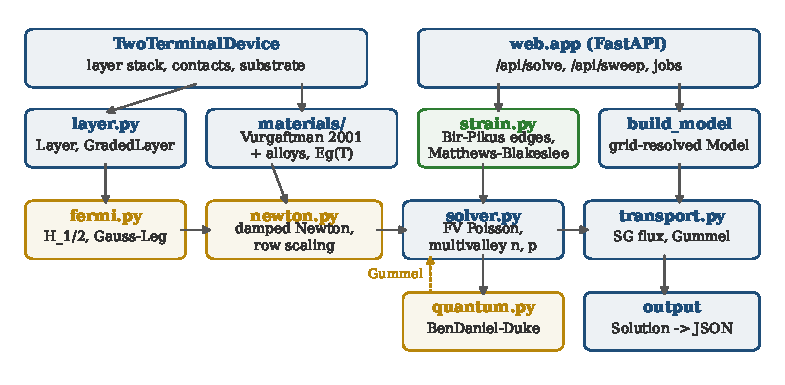
\includegraphics[width=\textwidth]{figures/fig_architecture.pdf}
\caption{Module map and data flow. A device description is flattened onto the
grid once (\texttt{build\_model}), optionally after strain has moved the band
edges; the three solvers then share that array set. Dashed arrow: the
quantised density is held fixed while Poisson is re-solved, which is the
Gummel loop of Section~\ref{sec:quantum}.}
\label{fig:architecture}
\end{figure*}

\subsection{Interface}

A calculation is described by a list of layers and two contacts. Doping is
signed---positive for acceptors, negative for donors---so that a $p$--$n$
junction reads as written on the wafer:

\begin{verbatim}
from obpds import Layer, OhmicContact, TwoTerminalDevice

dev = TwoTerminalDevice(
    [Layer(1000, "GaAs", Na=1e17),      # thickness in nm
     Layer(1000, "GaAs", Nd=1e17)],
    [OhmicContact(), OhmicContact()],
    T=300, N=1000, approx="kane")

sol = dev.get_equilibrium()             # band diagram
dd  = dev.get_drift_diffusion(0.8)      # dd.J in A/cm^2
V, J = dev.get_iv(-0.5, 1.0, 31)        # I--V sweep
V, C = dev.get_cv(-1.0, 0.3, 41)        # C--V sweep
\end{verbatim}

Pseudomorphic strain is a property of the wafer, not of a layer, so it is
given once at the device level and applied to every layer:

\begin{verbatim}
dev = TwoTerminalDevice([Layer(20, "GaAs", Nd=1e17),
                         Layer(8, "GaInAs", composition=0.8),
                         Layer(20, "GaAs", Nd=1e17)],
                        substrate="GaAs")
sol = dev.get_quantum_equilibrium(n_states=8)
sol.subbands["levels_eV"]           # bound levels, eV
sol.subbands["sheet_density_cm2"]   # 2DEG sheet density
\end{verbatim}

Band parameters can be calibrated per layer when the tabulated values do not
describe a particular sample:

\begin{verbatim}
well = Layer(8, "GaInAs", composition=0.8,
             overrides={"VBO": -0.42, "b_shear": -1.9})
\end{verbatim}

The valence-band offset and the strain parameters are the two things open to
override; the value replaces the unstrained parameter, so strain is applied on
top of it. Everything else feeds derived quantities---$n_i$, $N_c$, $N_v$, the
non-parabolicity---that would be left stale if half of a parameter set were
changed, and a misspelt key raises instead of being ignored.

All returned objects are plain attribute containers with an \texttt{as\_dict}
method that downsamples onto a common index set, which is what the web service
serialises. Operating points are cached by \texttt{(bias, T, N, approximation)}
so that repeated queries from an interactive session cost nothing.

\subsection{Browser front end}

The same solver is served by a FastAPI application (\texttt{obpds-web}, or
\texttt{uvicorn web.app:app}). The service exposes the presets, accepts a
device description as JSON, runs the solve in a worker thread and returns the
payload the front end draws: band edges per valley, quasi-Fermi levels, carrier
densities, field, the split valence edges when the stack is strained, subband
levels and wavefunctions when the quantum correction is on, and the terminal
current with its spread. The front end is deliberately dependency-free---SVG
drawn by hand, no framework---because the point of the workbench is that a
student can open a browser and see a band diagram without installing anything.
The service is not required for any of the numerics; it imports the library
and calls the same public methods as the script above.

A concrete exercise, of the kind the workbench was built for: load the
AlGaAs/GaAs HEMT preset with the quantum box ticked, then widen the well from
\SI{8}{nm} to \SI{12}{nm} and watch $E_0$ fall and the centroid move into the
well; or leave the geometry alone and raise the subband count, which shows how
many states a well of that depth actually binds before the levels cross
$E_{\rm cut}$. Neither needs an installation, and neither is easy to convey
in a static figure.

% =============================================================== 3 Model
\section{Physical models}
\label{sec:model}

\subsection{Notation and conventions}

Throughout, energies are in electron volts and the electrostatic potential
$\psi$ is in volts; the two are numerically equal for a single electron
charge, so a band edge bends as $E_c(x)=C(x)-\psi(x)$ with no separate
charge factor. The applied bias $V$ is the potential of the left/top contact,
the right/bottom contact being grounded, and the carrier quasi-Fermi levels
$F_n$, $F_p$ are energies in eV pinned to $-V$ and $0$ at the left contact
and to $0$ at the right. A positive $V$ therefore raises $F_n-F_p$ and is
forward bias for a diode with its $p$ region on the left. The current
densities $J_n$, $J_p$ are in A/cm$^2$ and are taken positive when the
corresponding carrier flows from left to right; the terminal current $J$
reported below is $J_n+J_p$. Doping is signed---positive for acceptors,
negative for donors---so $N_{\rm net}=N_D^{+}-N_A^{-}$.

\subsection{Electrostatics and carrier statistics}

With the electrostatic potential $\psi$ in volts (numerically equal to the
potential energy of an electron in eV), the Poisson equation is
\begin{equation}
  \frac{d}{dx}\!\left(\varepsilon(x)\frac{d\psi}{dx}\right)
  = -q\left[p - n + N_{\rm net}(x)\right],
  \label{eq:poisson}
\end{equation}
with $N_{\rm net}=N_D^{+}-N_A^{-}$ and Dirichlet conditions at the contacts.
The electron density is summed over the $\Gamma$, $L$ and $X$ valleys. For the
$\Gamma$ valley the Kane dispersion is used~\cite{Kane1957}, so that
\begin{equation}
  n_\Gamma = \frac{2}{\sqrt{\pi}}N_c^\Gamma\,
  H_{1/2}(\phi,\alpha), \qquad
  H_{1/2} = G_{1/2} + 2\alpha\,G_1,
  \label{eq:kane}
\end{equation}
where $G_k(\phi,\alpha)=\int_0^\infty t^k\sqrt{1+\alpha t}\,
[1+e^{t-\phi}]^{-1}dt$ and $\alpha=(kT/E_g)(1-m^{*}/m_0)^2$ is the
non-parabolicity parameter on the $kT$ scale. The $L$ and $X$ valleys are
treated as parabolic with their own densities of states and their own band
edges, so that a material that becomes indirect under strain or alloying moves
its electrons between valleys without a discontinuity. The holes use the
heavy-hole, light-hole and split-off masses, with the split-off band separated
by $\Delta_{\rm SO}$; under strain the three edges are no longer degenerate and
the density of states is reweighted (Section~\ref{sec:strain}).

The integrals in Eq.~\eqref{eq:kane} are evaluated by Gauss--Legendre
quadrature after the substitution $t=u^2$, which removes the $\sqrt{t}$
endpoint singularity in the derivative of the integrand; with 128 nodes and an
upper limit $u_{\max}=\sqrt{\max(\phi,0)+60}$ the values and their derivatives
with respect to $\phi$ come out of one pass over the nodes, which is what the
Newton Jacobian needs. The piecewise minimax rational approximations of
Fukushima~\cite{Fukushima2015} are more accurate still, but they carry a large
coefficient table for a gain that is invisible at the tolerance of a Newton
iteration. Against adaptive quadrature the median relative difference of the
quadrature is $1\times10^{-13}$ over $-5\le\phi\le15$; the single outlier,
$8\times10^{-10}$ at $\phi=-5$, is limited by the absolute tolerance of the
reference integral, whose value there is only $5\times10^{-3}$.

The band parameters are those of the Vurgaftman
compilation~\cite{Vurgaftman2001}, the dielectric constants those of
Adachi~\cite{Adachi2005}, and the temperature dependence of the gap is
Varshni's. A ternary is interpolated between its binaries with a bowing
parameter applied to the gap at the device temperature rather than at zero
temperature---a detail that moves In$_{0.53}$Ga$_{0.47}$As by
\SI{0.1}{eV} if it is got wrong.

\subsection{Pseudomorphic strain}
\label{sec:strain}

A layer thinner than its critical thickness cannot relax: it takes the in-plane
lattice constant of the substrate and compensates along the growth direction.
For growth along $[001]$ and a free surface ($\sigma_{zz}=0$),
\begin{equation}
  \varepsilon_\parallel = \frac{a_{\rm sub}-a}{a}, \qquad
  \varepsilon_\perp = -2\frac{C_{12}}{C_{11}}\varepsilon_\parallel,
  \label{eq:strain}
\end{equation}
so that $\mathrm{Tr}(\varepsilon)=2\varepsilon_\parallel+\varepsilon_\perp$.
The conduction band moves by the hydrostatic term, $\delta E_c =
a_c\,\mathrm{Tr}(\varepsilon)$, for all three valleys.

In the unstrained crystal the heavy- and light-hole edges coincide, so any
strain with a shear component resolves a degeneracy instead of perturbing a
single level. For a $[001]$ biaxial strain the Bir--Pikus Hamiltonian splits
into a diagonal $|3/2,\pm3/2\rangle$ block and a $2\times2$ block that mixes
$|3/2,\pm1/2\rangle$ with $|1/2,\pm1/2\rangle$ through the spin--orbit
coupling, and both diagonalise by hand. With
\begin{equation}
  h = a_v\mathrm{Tr}(\varepsilon), \quad
  d = -2b(\varepsilon_\perp-\varepsilon_\parallel), \quad
  s = \sqrt{\Delta^2-\Delta d+\tfrac{9}{4}d^2},
  \label{eq:bp}
\end{equation}
they are
\begin{equation}
  E_{\rm hh} = E_v + h + \frac{d}{2},\quad
  E_{\rm lh} = E_v + h - \frac{\Delta}{2} - \frac{d}{4} + \frac{s}{2},\quad
  E_{\rm so} = E_v + h - \frac{\Delta}{2} - \frac{d}{4} - \frac{s}{2}.
  \label{eq:edges}
\end{equation}
The closed form is worth having because it is checkable: at zero strain it reduces exactly to
$E_{\rm hh}=E_{\rm lh}=E_v$ and $E_{\rm so}=E_v-\Delta$; the shear part is
traceless, so the sum of the three edges is independent of $d$; and as
$\Delta\to\infty$ the heavy--light separation tends to $d$ with an error that
falls as $1/\Delta$. All three are assertions in the test suite
(Section~\ref{sec:verification}).

Sign conventions for the deformation potentials are a standing trap. We use
the Van de Walle--Chuang form~\cite{VandeWalle1989,Chuang1991} ($a_v>0$, gap
shift $(a_c-a_v)\mathrm{Tr}\,\varepsilon$); the Vurgaftman
compilation~\cite{Vurgaftman2001} tabulates $a_v$ with the opposite sign and
therefore writes the same shift as $(a_c+a_v)$. The parameter file declares
which convention it follows, and a regression test pins the hydrostatic
coefficient $dE_g/dP=-(a_c-a_v)/B$ at \SI{11.04}{meV/kbar} for GaAs, within
\SI{0.3}{meV/kbar} of the measured value.

Strain is applied only where it is defined: a layer with no deformation
potential in the parameter set (the nitrides) is still reported as strained
elastically, but its band edges do not move, and the layer table says so
instead of silently doing nothing. Layers thicker than the
Matthews--Blakeslee critical thickness~\cite{Matthews1974} are flagged, not
relaxed.

\subsection{Drift--diffusion transport}

The current is written in the thermodynamic form $J_n=q\mu_n n\,dF_n/dx$ and
$J_p=q\mu_p p\,dF_p/dx$, with $F_n$ and $F_p$ the quasi-Fermi levels in
eV~\cite{Selberherr1984,Lundstrom2000}.
Continuity is discretised in finite-volume form over a cell of width $h$,
\begin{equation}
  J_n|_{i+1/2}-J_n|_{i-1/2} = +qR_ih, \qquad
  J_p|_{i+1/2}-J_p|_{i-1/2} = -qR_ih,
  \label{eq:continuity}
\end{equation}
with the link fluxes given in Section~\ref{sec:sg}. Recombination is
Shockley--Read--Hall through mid-gap traps plus band-to-band radiative;
Auger is not included. Both quasi-Fermi levels are pinned to the metal level at
each contact, which is the ideal ohmic contact with infinite surface
recombination.

Two details of the recombination term decide whether it is right. The driving
force is $np-n_0p_0$, the departure from equilibrium, and not $np-n_i^2$:
under Fermi--Dirac or Kane statistics $np$ differs from $n_i^2$ by a few per
cent even at equilibrium, and that residual appears as a spurious generation
rate at zero bias. The trap densities are
$n_1=n_{\rm eff}e^{(E_t-E_i)/kT}$ and $p_1=n_{\rm eff}e^{(E_i-E_t)/kT}$ with
$n_{\rm eff}=\sqrt{n_0p_0}$, which generalises $n_i$ to whatever statistics are
in force; they are \emph{not} the local equilibrium densities. Substituting
$n_0$ and $p_0$ there is the tempting shortcut---it also makes $R$ vanish at
equilibrium---but it is equivalent to letting the trap energy slide with the
Fermi level, and in the depletion region it inflates the denominator by the
majority density, suppressing generation by two orders of magnitude. The
mistake hides well, because in the neutral regions both choices reduce to the
same minority lifetime and the forward knee looks correct; only the reverse
characteristic exposes it.

Mobilities are the tabulated room-temperature low-field values, scaled as
$(T/300)^{-1.5}$. There is no velocity saturation and no doping dependence:
those would need parameters that no III--V compilation provides consistently,
and inventing them would make the current look more authoritative than it is.

\subsection{Self-consistent quantisation}
\label{sec:quantum}

Classical electrostatics puts the electron gas exactly at the band-edge
minimum, which for a heterojunction is the interface plane. Confining a state
to a slab of thickness $L$ costs at least $\hbar^2\pi^2/2m^{*}L^2$ of kinetic
energy, so the ground state floats above the band edge and its wavefunction
has a lobe pushed away from the interface. A position-dependent mass makes the operator itself a choice, and only one
arrangement of it is Hermitian: the BenDaniel--Duke form~\cite{BenDaniel1966}
\begin{equation}
  -\frac{\hbar^2}{2}\frac{d}{dx}\!\left(\frac{1}{m^{*}(x)}
  \frac{d\varphi}{dx}\right) + E_c(x)\varphi = E\varphi,
  \label{eq:bd}
\end{equation}
It conserves the flux $(1/m^{*})d\varphi/dx$ through an interface, which the
naive $-\hbar^2\varphi''/2m^{*}+E_c\varphi$ does not. Discretised on the Poisson
grid, with $1/m^{*}$ averaged harmonically onto the faces,
Eq.~\eqref{eq:bd} is a symmetric tridiagonal eigenproblem.

A bound subband is a two-dimensional gas, so its sheet density is closed form,
because the two-dimensional Fermi--Dirac integral is a logarithm:
\begin{equation}
  N_i = \frac{m^{*}kT}{\pi\hbar^2}\ln\!\left[1+e^{(F-E_i)/kT}\right],
  \label{eq:2d}
\end{equation}
which stays exact in the degenerate limit. The volume density follows as
$n(x)=\sum_iN_i|\varphi_i(x)|^2$. States above the continuum threshold
$E_{\rm cut}$---the lower of the two contact band edges, $E_c(0)$ and
$E_c(L)$, since an electron above it can escape to a contact---are not
discarded: their
contribution is the three-dimensional density weighted by the regularised
incomplete gamma function,
\begin{equation}
  n_{\rm cont}(x) = n_{\rm 3D}(x)\,
  Q\!\left(\tfrac32, \frac{\max(0,E_{\rm cut}-E_c(x))}{kT}\right),
  \label{eq:cont}
\end{equation}
which reduces to the three-dimensional result far from the well and decays
inside it. The weight has a precise meaning in one limit, which is worth
stating because the generalisation is an approximation. In the Boltzmann
limit, counting only the three-dimensional states whose perpendicular kinetic
energy clears the threshold gives
$n_{\rm cont}(x)=n_{\rm 3D}(x)\,Q(3/2,(E_{\rm cut}-E_c)/kT)$, exactly: the
regularised incomplete gamma is the closed form of that integral, and the
subband sum plus this remainder then counts every electron once, so the
classical density is recovered far from the well and the bound states are not
double counted inside it. Under Fermi--Dirac statistics Eq.~\eqref{eq:cont}
is applied as a multiplicative weight on the *degenerate* density, which is
an approximation---the 2D subbands carry the physics of confinement and the
weight only has to be right in the crossover. The formula also assumes a
single threshold $E_{\rm cut}$ set by the lower contact edge, which is
exact for a symmetric device but an idealisation for asymmetric contacts or
multiple wells; those are not studied here. Without some such term the
density outside the well would vanish, so the approximation is kept and its
status recorded.

% ============================================================ 4 Numerics
\section{Discretisation and solvers}
\label{sec:numerics}

\subsection{Finite-volume Poisson}

Equation~\eqref{eq:poisson} is discretised in flux form on a node-centred
uniform grid, with the face permittivity taken as the harmonic mean of the two
adjacent nodes,
\begin{equation}
  \varepsilon_{i+1/2} = \frac{2\varepsilon_i\varepsilon_{i+1}}
  {\varepsilon_i+\varepsilon_{i+1}} .
  \label{eq:harmonic}
\end{equation}
For a piecewise-constant $\varepsilon$ whose jump lies between the two nodes,
the harmonic mean is the equivalent permittivity of two half-cells in series
and hence the coefficient that makes the discrete flux exact for that
assumption; node material parameters are assigned to the faces this way, and
it is what makes the discrete operator faithful to the un-expanded form of
Eq.~\eqref{eq:poisson}. Writing the
equation as $\varepsilon\psi''+\varepsilon'\psi'=-q\rho$ and then dropping the
second term, which is a common simplification, leaves a spurious field at every
heterointerface with a permittivity contrast; the harmonic mean retains it
without any special-casing.

The nonlinear system is solved by Newton's method with the damping of Bank and
Rose~\cite{BankRose1981}: the undamped step is computed, the residual ratio
$\xi=\|G(u+s\,\delta u)\|/\|G(u)\|$ is formed, the step is halved if the
reduction is smaller than $\tau s$, and otherwise accepted with the damping
factor updated as $s/(s+(1-s)\xi/2)$. The initial guess is not $\psi=0$: each
node is first solved for local charge neutrality with a scalar Newton
iteration, seeded from the Boltzmann expression and refined against the full
statistics, so that degeneracy, satellite valleys and non-parabolicity are
already accounted for before the global solve starts.

\subsection{A cancellation-free Scharfetter--Gummel flux via a generalised potential}
\label{sec:sg}

Exponential fitting requires the density to be exponential in a potential, and
the textbook derivation~\cite{Scharfetter1969} assumes Boltzmann statistics. Rather than accept that
restriction, define at every node the generalised potential
\begin{equation}
  \Psi_n \equiv F_n - kT\ln\frac{n}{N_{\rm ref}},
  \qquad
  \Psi_p \equiv F_p + kT\ln\frac{p}{N_{\rm ref}},
  \label{eq:psi}
\end{equation}
which is an identity for any statistics---parabolic Fermi--Dirac, Kane,
multi-valley---because it is built from the solved $n$ and $p$ themselves. In
the non-degenerate limit it reduces to $\Psi_n\to E_c-kT\ln(N_c/N_{\rm ref})$.
Because it is defined this way it carries the electrostatic potential, every
heterojunction band-edge step, the density-of-states gradients and the
degeneracy correction at once, and there is no separate band-gap-narrowing or
effective-field term to get wrong.

With $u=(\Psi_{i+1}-\Psi_i)/kT$ the standard link flux is
\begin{equation}
  J_n|_{i+1/2} = \frac{q\mu_n kT}{h}
  \left[n_{i+1}B(-u_n) - n_iB(u_n)\right],
  \qquad B(x)=\frac{x}{e^x-1}.
  \label{eq:sg}
\end{equation}
Written this way the two terms are each of order $\mu kT n/h$ and cancel to
order $\mu n\,dF/dx$; at equilibrium they differ in the sixteenth digit, which
for $\mu=\SI{8500}{cm^2\,V^{-1}\,s^{-1}}$, $n=10^{17}$~cm$^{-3}$ and
$h=\SI{10}{nm}$ is a
spurious current of $10^{10}$~A/cm$^2$. Substituting Eq.~\eqref{eq:psi} into
Eq.~\eqref{eq:sg} and using
$u_n=w_n-\ln(n_{i+1}/n_i)$ with $w_n=(F_{n,i+1}-F_{n,i})/kT$, the bracket
collapses analytically:
\begin{align}
  J_n|_{i+1/2} &= \frac{q\mu_n kT}{h}\,n_{i+1}B(-u_n)
  \left(1-e^{-w_n}\right),
  \label{eq:sgclean}\\
  J_p|_{i+1/2} &= \frac{q\mu_p kT}{h}\,p_iB(-u_p)
  \left(1-e^{-w_p}\right).
  \label{eq:sgcleanp}
\end{align}
The factor that vanishes at equilibrium is now computed from the quasi-Fermi
level itself, so $J=0$ at $w=0$ in floating point, with no cancellation
involved. This is the form the program uses.

Two statements must be kept apart, because only one of them is claimed here.
The identity between Eq.~\eqref{eq:sg} and
Eqs.~\eqref{eq:sgclean}--\eqref{eq:sgcleanp} is *algebraic*: substituting
Eq.~\eqref{eq:psi} into Eq.~\eqref{eq:sg} collapses the bracket exactly, for
any $n_{i+1}/n_i$, because the two terms are the same expression written in
different variables. That rearrangement neither introduces nor removes an
approximation, so it is safe for degenerate and non-parabolic carriers in the
same sense that Eq.~\eqref{eq:sg} itself is. What the rearrangement is *not*
is a proof that Eqs.~\eqref{eq:sgclean}--\eqref{eq:sgcleanp} are a consistent
discretisation of the continuous drift--diffusion equation under arbitrary
statistics: the exponential-fitting argument behind the Scharfetter--Gummel
flux assumes a Boltzmann density--potential relation, and the generalised
potential of Eq.~\eqref{eq:psi} is the device by which the same flux is
applied to other statistics. The truncation error of that application is not
established here and is a legitimate subject for a dedicated consistency
study; what we rely on is the residual, which is driven to the round-off
floor (Section~\ref{sec:continuity}).

The same caveat applies to the equilibrium statement. The flux is zero by
construction *when the stored quasi-Fermi levels satisfy $w=0$ exactly*; how
closely a converged solve approaches that condition is a property of the
solver's residual and of floating point, not of the formula. The verification
suite checks that a converged equilibrium solution returns zero current to
the reported tolerance (Section~\ref{sec:verification}), which is the honest
form of the claim.

\subsection{Continuity, damping and row equilibration}
\label{sec:continuity}

Each continuity equation is solved by Newton's method for one quasi-Fermi
level with the other frozen. The Jacobian is tridiagonal and is assembled
analytically, differentiating Eq.~\eqref{eq:sgclean} with $B(-u)$ lagged. The
lag is exact for Boltzmann statistics and an approximation otherwise: the
converged solution is therefore judged by the residual rather than by the
linearisation, and the residual tolerance is set below the quantity the
current is compared against (see below). We do not quantify the effect of
the lag on the convergence rate beyond the observation that a bias point
converges in two or three Gummel sweeps from a cold start
(Section~\ref{sec:gummel}); a rigorous convergence analysis of the
lagged-Jacobian linearisation is outside the scope of this work.

Semiconductor Jacobians span an extreme dynamic range: in the continuity
equations a neutral-region row is of order $\mu kT n/h\sim10^{27}$ while a
Dirichlet row is of order one, so the matrix is numerically singular although
it is well conditioned after equilibration. Since Newton's step is invariant
under left multiplication, dividing row $i$ of both the Jacobian and the
residual by the row infinity norm is a free preconditioner, and the program
does it. This matters more than it sounds: an earlier version measured the
residual after equilibration and declared convergence while the minority
carrier profile was flat and the current missing, because a residual that
looks tight in equilibrated units can still permit an imbalance a billion times
the quantity being solved for. The residual tolerance is therefore expressed
in physical units, at $10^{-16}$ of the equilibrated scale, which keeps the
current imbalance four decades below the current itself.

\subsection{The Gummel loops}
\label{sec:gummel}

Poisson, the two continuity equations and (optionally) the eigenvalue problem
are coupled by Gummel iteration~\cite{Gummel1964}. For transport, one sweep is:
solve Poisson with the quasi-Fermi levels frozen, then electron continuity,
then hole continuity; repeat until the largest change in $\psi$, $F_n$ or
$F_p$ falls below $10^{-7}$~eV.

The starting point is the part that decides whether this converges at all. In a
quasi-neutral region the minority density obeys $Dc''=(c-c_0)/\tau$, and since
the region is thin compared with the diffusion length the profile is very
nearly linear between the injected value $c_0e^{V/kT}$ at the depletion edge
and $c_0$ at the contact. Writing $c\propto e^{\pm F/kT}$ turns that straight
line into a logarithmic quasi-Fermi level,
\begin{equation}
  F(s) = F_{\rm majority} + kT\ln\!\left[e^{V/kT}(1-s)+s\right],
  \label{eq:start}
\end{equation}
with $s$ the fractional distance from the junction to the contact. The
expression is exact for either sign of $V$, because $e^{V/kT}$ is positive
however negative $V$ becomes; a formula built on $1-e^{-|V|/kT}$ instead
diverges as soon as the bias changes sign. Getting this shape right matters far
more than it looks: a linear ramp---the obvious guess---sits about
\SI{0.13}{V} away from the answer in the middle of the neutral region, and the
continuity Jacobian there is a near-Laplacian whose row sum is only
$\sim10^{-4}$, so that residual is amplified into a \SI{100}{V} Newton step
along a near-null direction and the solve is destroyed.

There is deliberately no bias continuation. Walking up from equilibrium looks
like the safe thing to do, but an ohmic contact pins the carrier
\emph{densities}, not the levels: reusing the previous operating point at a new
bias leaves the contact densities off by $e^{\Delta V/kT}$ and the first
nonlinear Poisson solve diverges. With the analytic start of
Eq.~\eqref{eq:start} a bias point converges in two or three sweeps from cold,
so there is nothing for continuation to save, and every bias point is
independent---which also makes an I--V sweep trivially parallel.

The quantum loop is the same idea with the density replaced: solve the
eigenproblem on the current band edge, rebuild $n$ from Eqs.~\eqref{eq:2d}
and \eqref{eq:cont}, re-solve Poisson with that density held fixed, repeat.
Holding the density fixed is what makes this a Gummel iteration rather than a
coupled Newton solve; the price is linear convergence, the reward is that each
step is a well-conditioned Poisson problem. Undamped, the map turns out to be a
contraction, with the potential change falling by a factor of about $0.78$ per
sweep, because the feedback is self-limiting: pushing electrons off the
interface lowers the field there, which shallows the well, which pushes them
back. Damping is kept only as a safety net, applied when a sweep makes the
residual worse.

The quantum loop is run at equilibrium only. There is no quantum-corrected
drift--diffusion: the I--V curve, the C--V curve and the current of
Section~\ref{sec:results} are all classical, and the subband structure is a
property of the zero-bias band profile.

\subsection{The eigenproblem}

Three details of the discretisation decide whether the spectrum is right, and
none of them shows up in a plot of the wavefunction.

\emph{Walls.} The zero condition is imposed on a ghost node one step outside
the grid. Its value never enters the matrix, but its flux does, on the diagonal
of the first and last rows. Dropping that term makes the wall reflecting: every
level falls by about one mesh step and a state appears near $E\approx0$, so a
triangular well returns less than half its true ground-state energy.

\emph{Inner product.} The assembled operator is self-adjoint under the nodal
sum, which fixes the normalisation to
$\|\varphi\|=(\sum_i\varphi_i^2)^{1/2}\sqrt{h}$. Weighting the nodes
trapezoidally belongs to a different inner product and leaves the Gram matrix
orthogonal only to $10^{-6}$, against $10^{-16}$ for the nodal sum.

\emph{Interface mass.} The mass sits inside the derivative in
Eq.~\eqref{eq:bd}, so two half-cells in series combine harmonically, as the
permittivity does in Eq.~\eqref{eq:harmonic}. An arithmetic average of
$1/m^{*}$ is the common shortcut, and it costs the matrix its symmetry.

The eigenvalues come from \texttt{eigh\_tridiagonal}, a symmetric-tridiagonal
solver asked for the lowest few states by index: one tridiagonal
factorisation replaces a full spectrum. The density-of-states mass of a
subband is the in-plane mass, and a state that straddles an interface samples
both materials, so it is taken as the $|\varphi|^2$-weighted average rather
than the mass at whichever node happens to be the well bottom.

\subsection{Reading the terminal current}

$J_n+J_p$ is constant in exact arithmetic, but its discrete value is not
equally trustworthy everywhere. A majority carrier in a quasi-neutral region
carries the current as $q\mu c\,dF/dx$ with $c\sim10^{17}$~cm$^{-3}$, so the
gradient belonging to a $10^{-15}$~A/cm$^2$ current is $\sim10^{-22}$~eV per
cell---five orders of magnitude below the round-off of a stored level of order
$0.1$~eV. Those links report pure noise. Inside the depletion region both
carriers are minorities, both densities are near $n_i$ and both fluxes are
clean, so the program reads the terminal current as the median of $J_n+J_p$
over the links where $\max(n,p)\le10^{3}n_i$. If no link satisfies that
criterion---at high forward bias the depletion region fills with carriers and
none does---the median is taken over the whole device, and
\texttt{J\_spread} then states how little the number deserves to be trusted.
It reports
\begin{equation}
  \texttt{J\_spread} = \frac{\max_k|J_k-J|}{|J|},
  \label{eq:spread}
\end{equation}
the relative deviation of the worst link. Two clarifications are in order,
because both were misread in review. First, \texttt{J\_spread} is a
*diagnostic*, not an error bar: it tells the user when the reported value is
dominated by round-off, but it is not a bound on the true current, and no
such bound is claimed. Second, the median rule is a device for reading a
nearly constant quantity off a noisy vector, and it is insensitive to the
threshold: the reported current changes by less than one part in $10^{10}$
when the $10^{3}n_i$ cutoff is moved to $10^{2}n_i$ or $10^{4}n_i$
(Table~\ref{tab:current}). At \SI{0.8}{V} forward bias \texttt{J\_spread} is
$1.9\times10^{-4}$, at \SI{-1}{V} it is $373$: the reverse current of this
device is not resolvable beyond its leading digits at $N=1000$, and the
program says so instead of printing six figures.

An independent check, using quantities the median rule does not touch,
confirms that reading. Integrating the discrete continuity equation over the
device, the terminal current must satisfy
$J_{\rm left}-J_{\rm right}=q\int R\,dx$. Table~\ref{tab:current} reports
this balance: at \SI{0.8}{V} the two sides agree to $2.6\%$ of the current,
but the imbalance grows to $50\%$ at \SI{0.6}{V}, $126\%$ at \SI{0.4}{V} and
roughly $200\%$ in reverse bias. Where the conservation residual is a large
fraction of the current, no choice of reading point can recover a meaningful
number, and the paper restricts its quantitative I--V claims to the bias
range where the balance holds; below that the characteristic is qualitative.

\begin{table}[t]
\centering
\caption{Current reporting for the GaAs $p$--$n$ junction at $N=1000$:
the median of $J_n+J_p$ over links with $\max(n,p)\le k\,n_i$, and the
continuity-balance check $J_{\rm left}-J_{\rm right}$ against
$q\int R\,dx$. The median is insensitive to the threshold $k$; at $+0.4$~V and
above no link satisfies the criterion (the depletion region has filled), so
the median falls back to the whole device. The balance is the independent
evidence that the low-bias current is below the arithmetic noise floor.}
\label{tab:current}
{\small
\setlength{\tabcolsep}{4pt}
\begin{tabular}{@{}lrrrrr@{}}
\toprule
$V$ (V) & $J$ (A/cm$^2$) & spread & $k=10^3$ median & balance (rel.) \\
\midrule
$+0.8$ & $3.32\times10^{-4}$ & $1.9\times10^{-4}$ & $3.32\times10^{-4}$ & $0.026$ \\
$+0.6$ & $2.83\times10^{-7}$ & $1.2\times10^{-2}$ & $2.83\times10^{-7}$ & $0.50$ \\
$+0.4$ & $2.57\times10^{-9}$ & $0.42$ & $2.57\times10^{-9}$ & $1.26$ \\
$-0.5$ & $-5.29\times10^{-12}$ & $335$ & $-5.29\times10^{-12}$ & $2.00$ \\
$-1.0$ & $-9.50\times10^{-12}$ & $373$ & $-9.50\times10^{-12}$ & $2.00$ \\
\bottomrule
\end{tabular}}
\end{table}

% ========================================================= 5 Verification
\section{Verification}
\label{sec:verification}

\subsection{Strategy}

The program is held to closed-form results, not to itself. Three suites and
an end-to-end API test carry the checks of Table~\ref{tab:suites}. The checks
are reported by kind rather than as a single undifferentiated count, because
the kinds prove different things: an analytic-limit check pins a physical
model against a closed form, a discrete-operator check pins a property of the
discretisation itself, and a physical-scale check catches a result in the
wrong decade without a closed form to compare against. The API test checks
the payload contract between the service and the front end, which is not a
physics assertion at all. Every tolerance is stated in the test source, and
every reference value is either an analytic expression or a literature number
with its provenance in a comment. The counts below are the number of
assertions the current revision of the suite executes; they change as tests
are added, so the source is the authority, not this table.

\begin{table}[t]
\centering
\caption{Verification suites and what their checks prove. ``Analytic'' are
closed-form or asymptotic limits; ``operator'' are properties of the discrete
operator (orthonormality, exact conservation, identities); ``scale'' are
physical-order-of-magnitude checks without a closed form; ``contract'' are
web-API payload checks, which are not physics assertions. The check count is
what the current revision executes; it grows as tests are added, so the test
source is the authority. Wall times are for one core of the machine described
in Section~\ref{sec:performance}.}
\label{tab:suites}
{\small
\setlength{\tabcolsep}{4pt}
\begin{tabular}{@{}lrlp{4.4cm}@{}}
\toprule
Suite & Checks & Kinds & Scope \\
\midrule
\texttt{validate\_physics.py} & 14 & analytic, operator &
  depletion approximation, short-base diode law, ideality factor,
  $1/\tau$ scaling, zero current \\
\texttt{validate\_quantum.py} & 32 & analytic, operator, scale &
  square, triangular and mass-step wells, 2D population limits,
  self-consistent loop \\
\texttt{validate\_strain.py} & 72 & analytic, operator &
  strain tensor, Bir--Pikus identities, pressure coefficient,
  critical thickness \\
\texttt{web\_smoke.py} & 82 & contract &
  API contract, every preset, every payload field \\
\midrule
Total & 200 & & \\
\bottomrule
\end{tabular}}
\end{table}

\begin{figure}[t]
\centering
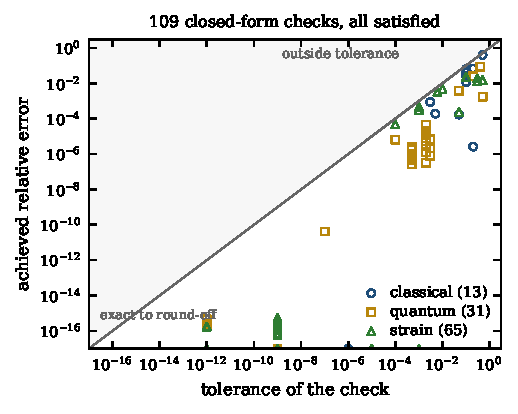
\includegraphics[width=\columnwidth]{figures/fig_verification.pdf}
\caption{Achieved relative error of each closed-form check against the
tolerance it is held to, for the three physics suites. Every point lies below
the diagonal; the cluster on the bottom axis is exact to round-off. The 81 API
assertions of \texttt{web\_smoke.py} check payload consistency rather than
physics and are not shown.}
\label{fig:verification}
\end{figure}

\subsection{Classical electrostatics and transport}

For a GaAs $p$--$n$ junction with $10^{17}$~cm$^{-3}$ on both sides
($n_i=1.70\times10^{6}$~cm$^{-3}$ at \SI{300}{K}) the built-in potential is
reproduced to $8.7\times10^{-4}$ relative, the depletion width inferred from
$2V_{\rm bi}/E_{\max}$ to $2.7\%$, and the peak field to $2.6\%$; the
deviations are those of the depletion approximation itself, which the
simulation is not obliged to obey. The integral of the net charge over the
device is $1.5\times10^{-21}$~C/cm$^2$.

For the current, the checks are the ones a diode obeys. The short-base diode
law $J=qn_i^2(D_n/W_pN_A+D_p/W_nN_D)e^{V/kT}$ is reproduced to $6.3\%$,
$4.7\%$ and $4.0\%$ at \SI{0.80}{V}, \SI{0.85}{V} and \SI{0.90}{V}; the local
ideality factor is $1.01$ in the diffusion regime and $1.92$ in the
SRH-dominated regime, the textbook two-region crossover; the reverse current
scales as $1/\tau$ with the ratio $9.99997$ for a decade change in lifetime;
and the equilibrium current is zero to the reported tolerance (the
cancellation-free form makes it zero by construction at $w=0$, and the solve
returns it to round-off). Current conservation at
\SI{0.8}{V} holds to $1.9\times10^{-4}$, which is the \texttt{J\_spread} of
that operating point. The reverse generation current at \SI{-0.5}{V} is
$5.3\times10^{-12}$~A/cm$^2$ against $8.7\times10^{-12}$~A/cm$^2$ from the
generation-volume estimate, a $39\%$ agreement---as good as that estimate,
which assumes a sharp depletion edge, can be.

The Kane statistics are checked where they matter: for InAs
($\alpha=0.070$) the non-parabolic integral exceeds the parabolic one by
$28.7\%$ at $\phi=2$, and the three approximations (Boltzmann, parabolic
Fermi--Dirac, Kane) agree in the non-degenerate limit and diverge as they
should as the density approaches the band.

\subsection{Quantisation}

An infinite square well reproduces $\hbar^2\pi^2n^2/2m^{*}L^2$ to
$3\times10^{-7}$ at $N=1601$, with second-order convergence in the mesh. A
triangular well reproduces the Airy zeros to $2.6\times10^{-7}$ once the
analytic reference is evaluated at the position of the ghost wall, $x=-h$,
the residual difference from evaluating it at $x=0$ is a constant
$Fh=\SI{0.1}{meV}$, a property of the discretisation. The mass-step well is the check
that actually tests the variable-mass form: the solver reproduces the
transcendental condition obtained from Eq.~\eqref{eq:bd} with the
BenDaniel--Duke interface condition to $7\times10^{-7}$, whereas a one-sided
numerical derivative is only first-order accurate and cannot distinguish the
correct formulation from a wrong one. The eigenfunctions are orthonormal to
$4\times10^{-16}$.

The two-dimensional population, Eq.~\eqref{eq:2d}, is checked in both limits:
$4\times10^{-11}$ against the Boltzmann expression and $7\times10^{-6}$ against
the degenerate asymptotic form.

\subsection{Strain}

The three identities of Section~\ref{sec:strain} are asserted for four
materials at four strain values: the zero-strain limit is exact to
$10^{-12}$, the shear part is traceless to $6\times10^{-16}$~eV, and the
$\Delta\to\infty$ limit converges to $d$ with the measured order $2.00$ in
$1/\Delta$ (errors $4.7\times10^{-3}$, $4.7\times10^{-4}$,
$4.7\times10^{-5}$ for $\Delta=10$, $100$, $1000$~eV). The hydrostatic
pressure coefficient lands at \SI{11.04}{meV/kbar} for GaAs and
\SI{10.49}{meV/kbar} for InAs. In$_{0.53}$Ga$_{0.47}$As on InP is lattice
matched to $3\times10^{-4}$, and the critical thickness decreases
monotonically with mismatch, from \SI{41.3}{nm} at $0.5\%$ to \SI{1.98}{nm} at
$4\%$.

The calibration interface of Section~\ref{sec:structure} is checked in the
same suite, because a half-applied parameter change is worse than none:
shifting a layer's valence-band offset by \SI{0.1}{eV} moves its conduction
edges by exactly the same amount and leaves the gap untouched to
$10^{-12}$~eV; overriding $a_c$ to zero removes the hydrostatic shift and
nothing else; and a misspelt key, or one that would leave derived quantities
stale, raises instead of being silently ignored.

\subsection{Negative controls}

Three checks are there to catch a correction that adds something where nothing
should be added, which is the failure mode of a quantisation scheme.

\emph{A classical junction must come back unchanged.} On a GaAs $p$--$n$
junction the quantum and classical densities agree to zero---bit for bit, at
$N=400$---and the solver finds no bound state at all, because
$E_{\rm cut}$ lies below every level. If the subband and continuum pieces
double counted or dropped density, this test would fail immediately.

\emph{A layer on its own substrate must not be strained.} Setting the
substrate to the layer material gives zero strain, zero valence shift and an
unchanged band offset.

\emph{The equilibrium current must vanish.} It does, by construction of
Eq.~\eqref{eq:sgclean} at $w=0$, and the assertion is kept because the
construction is easy to break.

\subsection{The API contract}

The 82 checks of \texttt{web\_smoke.py} post every preset through the
service and check the payload the front end actually draws: that each field the
browser reads is present and finite, that the arrays share one index set, that
the subband populations sum to the reported sheet density, that one
wavefunction is returned per bound state and that its length matches the grid,
and that the electron column contains the quantum density rather than the
classical one. This is the class of bug that a physics test cannot catch and a
user notices immediately, and it is cheap to keep covered.

% ============================================================ 6 Results
\section{Representative calculations}
\label{sec:results}

\subsection{A $p$--$n$ diode}

Figure~\ref{fig:iv} shows the I--V characteristic of the GaAs junction used
above, over eight decades of current, with the local ideality factor
$n=(q/kT)^{-1}dV/d\ln J$. The two regimes are cleanly separated: $n\simeq1.9$
below \SI{0.35}{V}, where recombination in the depletion region dominates, and
$n\simeq1.01$ above \SI{0.7}{V}, where diffusion in the neutral regions does.
The reverse current is flat to within the noise floor discussed in
Section~\ref{sec:performance}---a feature of the model (no avalanche, no
tunnelling) as much as of the solver.

\begin{figure*}[t]
\centering
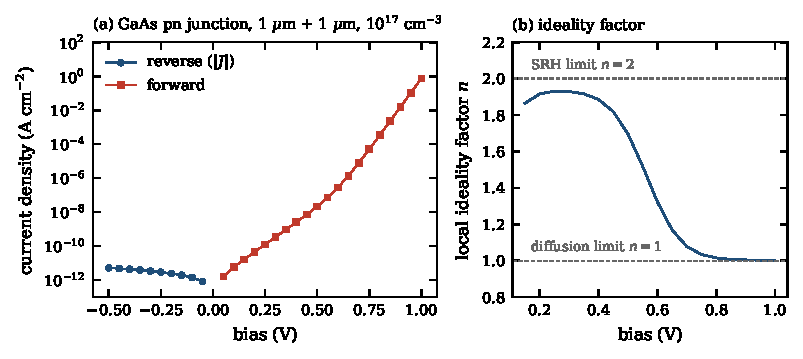
\includegraphics[width=\textwidth]{figures/fig_iv.pdf}
\caption{(a) Current density of the GaAs $p$--$n$ junction against bias.
(b) Local ideality factor, showing the SRH-limited and diffusion-limited
regimes. The values at the two plateaux are $1.92$ and $1.01$.}
\label{fig:iv}
\end{figure*}

\subsection{A modulation-doped heterojunction}

The second structure is the one the quantum correction exists for: \SI{30}{nm}
of Al$_{0.3}$Ga$_{0.7}$As doped at $10^{18}$~cm$^{-3}$, a \SI{10}{nm} undoped
spacer, and \SI{500}{nm} of GaAs. Donors in the barrier spill electrons into
the GaAs, where they collect in a notch narrow enough to quantise.

At $N=800$ the self-consistent loop converges to a single bound subband with
$E_0-E_{c,\min}=\SI{64.8}{meV}$, a sheet density of
$6.49\times10^{11}$~cm$^{-2}$, and a $|\varphi_0|^2$ centroid \SI{4.6}{nm}
behind the potential minimum (Figure~\ref{fig:hemt}). The classical solution
puts its peak at the minimum itself. The subband energy sits \SI{25}{\%} below
the bare-triangular estimate at the same field
(\SI{86.3}{meV} at $F=9.4\times10^{4}$~V/cm), which is the expected direction:
the well is not a bare triangle, because the charge that fills it flattens the
field.

\begin{figure*}[t]
\centering
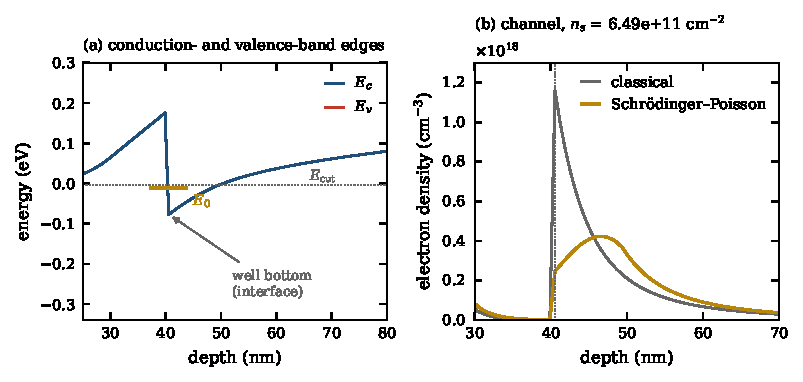
\includegraphics[width=\textwidth]{figures/fig_hemt.pdf}
\caption{(a) Band edges of the modulation-doped heterojunction with the bound
subband marked; $E_{\rm cut}$ is the continuum threshold of
Eq.~\eqref{eq:cont}. (b) Electron density near the interface: the classical
solution peaks at the potential minimum, the Schr\"odinger--Poisson solution
peaks \SI{4.6}{nm} behind it.}
\label{fig:hemt}
\end{figure*}

The total electron sheet density of the structure is $2.9\times10^{12}$~cm$^{-2}$,
of which only $6.5\times10^{11}$~cm$^{-2}$ is in the channel; the rest remains
in the doped barrier. That is the correct physics for a single heterojunction
with a \SI{30}{nm} doped barrier, and it is a reminder that the sheet density
reported for a "2DEG" is only the channel part if the structure is designed so.

\subsection{A strained well}

An In$_{0.2}$Ga$_{0.8}$As layer on GaAs is mismatched by $+1.43\%$; the wafer
locks it to $\varepsilon_\parallel=-1.413\%$ in plane, and it answers with
$\varepsilon_\perp=+1.317\%$ along the growth direction. The valence edge
splits by \SI{78.9}{meV}, heavy hole up. The bare shear parameter is
$d=\SI{93.9}{meV}$, so a calculation that left the spin--orbit coupling out
would put the light hole \SI{19}{\%} too low. The critical thickness is
\SI{10.15}{nm}: an \SI{8}{nm} well is pseudomorphic, a \SI{20}{nm} one is
flagged. The gap opens from \SI{1.1324}{eV} to \SI{1.2043}{eV} and the
conduction edge rises by \SI{101.9}{meV}, both of which move the confinement.

% ======================================================= 7 Performance
\section{Performance and the limits of the numbers}
\label{sec:performance}

\subsection{Cost}

Figure~\ref{fig:cost} reports wall times on one core of an Intel Core
i7-12700, Windows 11, Python 3.13.5, NumPy 2.5.4, SciPy 1.18.1. Each timing
is the \emph{median} of several repeats, with the min--max spread recorded in
\texttt{bench.json} alongside it, so the numbers are a typical runtime rather
than a best case; the cheap solves repeat five times, the expensive ones
three. The nonlinear
Poisson solve at $N=1000$ takes \SI{0.34}{s} (spread \SI{0.34}{s}--
\SI{0.37}{s}) and scales between linear and
quadratic in $N$; a drift--diffusion bias point takes \SI{1.47}{s} in two
Gummel sweeps; a full I--V point, cold-started and including the harder reverse
and high-forward biases, averages \SI{3.8}{s}; and a quantum equilibrium solve
for the heterojunction takes \SI{22.7}{s} (spread \SI{22.5}{s}--
\SI{24.7}{s}). These are single-core numbers on a problem of a few thousand
unknowns; nothing here needs a cluster, and an I--V sweep parallelises
trivially because the bias points are independent.

Almost all of the quantum cost sits in one kernel. A profile of the $N=800$
case puts $82\%$ of the runtime in the Fermi--Dirac quadrature: 7956
evaluations of four integrals over 128 nodes, for 58 Poisson solves. The node
count is deliberate---64 nodes would halve the time but is only good to
$6\times10^{-6}$ relative, and a quadrature error propagates straight into the
current. Batching the three valleys into one call and tabulating $H_{1/2}$ in
$\phi$ are the obvious levers and are left for a later version. The timings,
the machine and the library versions are written by \texttt{benchmark.py} into
the JSON that generated Fig.~\ref{fig:cost}, so each number is traceable to a
specific run.

\begin{figure*}[t]
\centering
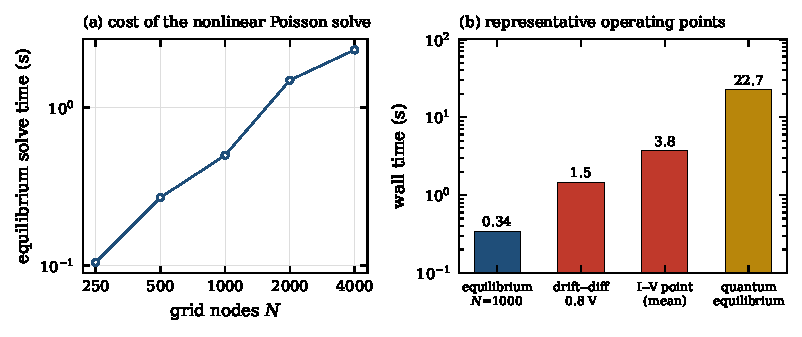
\includegraphics[width=\textwidth]{figures/fig_cost.pdf}
\caption{(a) Cost of the nonlinear Poisson solve against the number of grid
nodes. (b) Representative operating points. Numbers above the bars are seconds.}
\label{fig:cost}
\end{figure*}

\subsection{Accuracy limits, and saying so}

Two numerical limits are worth stating explicitly, because both are invisible
in a plot and both are properties of the discretisation rather than of the
physics.

The first is the current noise floor. Figure~\ref{fig:noise} shows the reported
current against the worst discrete link at each bias. At \SI{0.8}{V} the spread
is $1.9\times10^{-4}$; at \SI{0.4}{V} it is $0.42$; at \SI{-1}{V} it is $373$.
The interpretation is straightforward: above about \SI{0.6}{V} the reported
current is meaningful to the digits shown, at \SI{0.4}{V} only the leading
digit is, and below \SI{0.1}{V} the number is round-off. The program reports the diagnostic because a
minority-carrier device at low bias is exactly where a user is most likely to
believe a number that the arithmetic cannot support.

\begin{figure}[t]
\centering
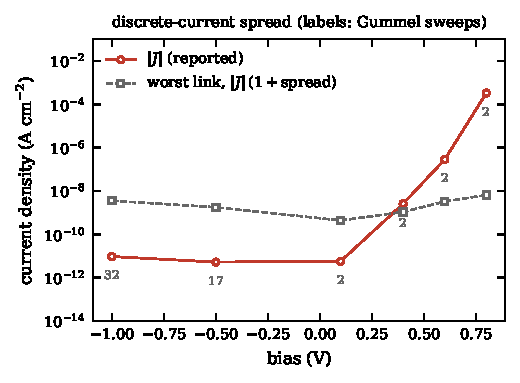
\includegraphics[width=\columnwidth]{figures/fig_noise.pdf}
\caption{Reported current density and the worst discrete link against bias for
the GaAs $p$--$n$ junction at $N=1000$. Labels give the number of Gummel sweeps.
Where the two curves converge, the discrete current is consistent; where they
separate, the reported value is dominated by round-off in the quasi-neutral
regions.}
\label{fig:noise}
\end{figure}

The second is the mesh sensitivity of the quantised sheet density. For the
heterojunction of Section~\ref{sec:results} the sheet density is
$7.28\times10^{11}$~cm$^{-2}$ at $N=400$, $6.49\times10^{11}$~cm$^{-2}$ at
$N=800$, $6.46\times10^{11}$~cm$^{-2}$ at $N=1600$ and
$6.60\times10^{11}$~cm$^{-2}$ at $N=3200$: about $12\%$ between the two
coarsest meshes, but the sequence is then *not* monotonic---the finest mesh
sits $2.2\%$ above the $N=1600$ value. A Richardson extrapolation of the
three finest meshes returns $6.72\times10^{11}$~cm$^{-2}$ with an observed
order of only $\sim0.5$, far from the second-order one would expect of the
discretisation, which signals that the error is not dominated by a smooth
$h$-power. The likely source is the well geometry: as the grid changes, the
interface node and the well width move by a fraction of a cell, and the
bound-state energy and its population respond to that discrete movement
rather than to the cell size. The ground-state energy behaves the same way:
\SI{-16.8}{meV}, \SI{-12.1}{meV}, \SI{-11.9}{meV}, \SI{-12.8}{meV} at the
four meshes. The default $N=1000$ is adequate for the sheet density to a few
per cent; the manuscript's earlier three-significant-digit quotes at $N=800$
are accordingly retired, and the values in Section~\ref{sec:results} should
be read to two significant digits. The audit script
\texttt{quantum\_convergence.py} writes the full table, and
\texttt{paper/cpc/data/qconv.json} carries it.

\subsection{What the model does not contain}

The following are outside the model, and are listed so that the numbers above
are read at their proper scope. The model is one-dimensional and isothermal; the transport is
drift--diffusion with constant low-field mobilities, with no velocity
saturation, no inter- or intra-valley scattering and no energy transport; holes
are not quantised, so the valence-band figures are edge splittings and not
valence subbands; the quantum correction is applied at equilibrium only, so no
current or capacitance reported here includes it; there is no exchange--correlation correction to the confined
gas; strain relaxation is reported, not modelled; the piezoelectric charge is
absent, which for $[001]$ growth is exact, because
a biaxial strain on that orientation has no shear component; the same $a_c$ is
used for the $\Gamma$, $L$ and $X$ valleys and the shear deformation potential
$\Xi_u$ is omitted; effective masses do not change with strain; and there is no
Auger recombination.

One disagreement with experiment is worth recording, because it propagates
into the device numbers above. For strained In$_x$Ga$_{1-x}$As wells our
conduction-band offset at $x=0.10$ is \SI{41}{meV}, against \SI{82}{meV} from
the capacitance--voltage determination of Zubkov \emph{et
al.}~\cite{Zubkov2004}, which fits $\Delta E_C=0.85x-0.3x^2$~eV---a factor of
two, systematic in $x$. Part of it is expected, because a C--V offset is
extracted with an assumed effective mass and an assumed well width that
correlate with the offset, but a factor of two is too large to attribute to
that alone. To see which parameter carries it, we perturb each strained-band
input the model consumes and record the resulting offset, gap, subband energy
and sheet density (Table~\ref{tab:strain_sens}, produced by
\texttt{strain\_sensitivity.py}). The valence-band offset is the dominant
lever: a shift of $-40$~meV moves the $x=0.10$ offset from \SI{41}{meV} to
\SI{81}{meV}, i.e.\ onto the Zubkov value, and changes the sheet density of
the Section~\ref{sec:results} well by up to a factor of four. The hydrostatic
deformation potential $a_c$ is the second lever, moving the offset by
$\pm20$~meV under a $\pm20\%$ rescaling and the sheet density by a factor
$\sim2.4$. The shear potential $b$ and the hydrostatic valence potential
$a_v$ leave the conduction-band offset unchanged, as they must, and affect
only the gap and the valence splitting. The conclusion is therefore a
bounded one: *for the tabulated parameter set*, the offset is \SI{41}{meV},
and the disagreement with C--V is within the range a plausible recalibration
of the valence-band offset explains, but the subband energies and sheet
densities of any strained-well calculation inherit that parameter
uncertainty. We report the comparison, and the override interface of
Section~\ref{sec:structure} exists so that a reader who prefers a different
valence-band offset can supply it per layer and watch what it does to the
offset, the subband energies and the sheet density, without touching the
parameter tables.

\begin{table}[t]
\centering
\caption{Strain-parameter sensitivity of the In$_{0.2}$Ga$_{0.8}$As/GaAs
well (Ga fraction $0.80$): conduction-band offset $dE_c$ (well relative to
the GaAs barrier), gap, sheet density and ground level, as each parameter is
shifted. A negative $dE_c$ means the well edge lies below the barrier.}
\label{tab:strain_sens}
{\small
\setlength{\tabcolsep}{4pt}
\begin{tabular}{@{}lrrrr@{}}
\toprule
Parameter & change & $dE_c$ (meV) & $n_s$ (cm$^{-2}$) & $E_0$ (meV) \\
\midrule
baseline & --- & $-85$ & $5.6\times10^{11}$ & $-11.5$ \\
VBO & $-20$~meV & $-105$ & $8.5\times10^{11}$ & $-29.9$ \\
VBO & $-40$~meV & $-125$ & $1.19\times10^{12}$ & $-48.7$ \\
VBO & $-80$~meV & $-165$ & $2.21\times10^{12}$ & $-86.0$ \\
$a_c$ & $\times0.8$ & $-106$ & $8.5\times10^{11}$ & $-30.3$ \\
$a_c$ & $\times1.2$ & $-65$ & $3.5\times10^{11}$ & $+6.0$ \\
$a_v$, $b$ & $\times0.8$--$1.2$ & $-85$ (unchanged) & $5.6\times10^{11}$ & $-11.5$ \\
\bottomrule
\end{tabular}}
\end{table}

% ========================================================== 8 Conclusions
\section{Conclusions}
\label{sec:conclusions}

OBPDS 2.0 is a one-dimensional solver for III--V heterostructures that
computes band diagrams, terminal currents, capacitances and quantised subband
structure on one grid, with pseudomorphic strain as a device-level property.
It is a derivative of a program that stopped at the zero-current
approximation; the additions are drift--diffusion transport, self-consistent
quantisation and strain, and the numerical work that makes them correct in a
material system whose carrier densities span more than twenty decades.

The parts we would point a reader to are the ones where the straightforward
implementation goes wrong in a way that looks right. A Scharfetter--Gummel flux
written in generalised potentials and rearranged to be cancellation-free gives
a zero equilibrium current, where the textbook form gives
$10^{10}$~A/cm$^2$ of numerical noise; the rearrangement is an algebraic
identity, and we have been careful to say so rather than claim a new
discretisation. Row equilibration of the continuity
Jacobian, with the residual tolerance expressed in physical rather than
equilibrated units, is the difference between a converged minority profile and
a flat one. A ghost-node flux, a nodal-sum normalisation and a harmonic
interface mass are three lines of code that decide whether the spectrum is
right. And in III--V materials the terminal current of a quasi-neutral region
is below the round-off of the stored levels, so the current has to be read
where it is clean and its spread reported.

All of this is held to a verification suite whose checks are reported by
kind---analytic and asymptotic limits, discrete-operator properties, and
physical-scale regression, plus a separate web-API contract test---including
the negative controls that make a quantisation scheme believable. The
program runs a representative bias point in about a second, is served by a
browser front end for classroom use, and is released under the same licence as
the work it derives from.

%% ------------------------------------------------------------- declarations
\section*{CRediT authorship contribution statement}
First Author: Conceptualization, Methodology, Software, Validation, Writing --
original draft. Second Author: Formal analysis, Investigation, Writing --
review \& editing.

\section*{Declaration of competing interests}
The authors declare that they have no known competing financial interests or
personal relationships that could have appeared to influence the work reported
in this paper.

\section*{Declaration of generative AI and AI-assisted technologies}
Generative AI tools were used to draft and refactor code and to prepare a
first draft of the manuscript text. The authors reviewed and edited the
content, ran all calculations, and take full responsibility for the published
work.

\section*{Data availability}
The program source, the verification suites, the scripts that regenerate every
figure and table of this article, and the raw output of every run are archived
in the CPC Program Library and at \url{https://doi.org/10.5281/zenodo.XXXXXXX}
under AGPL-3.0-or-later.

\section*{Acknowledgements}
This work reuses and extends the Open Band Parameters Device
Simulator~\cite{Maddox2015}, distributed under AGPL-3.0; the derived code is
released under the same licence. We thank the original author for making it
available.

\bibliographystyle{elsarticle-num}
\bibliography{refs}

\end{document}
